%% This Beamer template is based on the one found here: https://github.com/sanhacheong/stanford-beamer-presentation, and edited to be used for Stanford ARM Lab

\documentclass[10pt]{beamer}
%\mode<presentation>{}

\usepackage{media9}
\usepackage{amssymb,amsmath,amsthm,enumerate}
\usepackage{mathtools}
\usepackage[utf8]{inputenc}
\usepackage{array}
\usepackage[parfill]{parskip}
\usepackage[utf8]{vietnam}
\usepackage{graphicx,animate}
\usepackage{caption}
\usepackage{subcaption}
\usepackage{bm}
\usepackage{amsfonts,amscd}
\usepackage[]{units}
\usepackage{listings}
\usepackage{multicol}
\usepackage{multirow}
\usepackage{tcolorbox}
\usepackage{physics}
\usepackage{movie15}
% Enable colored hyperlinks
\hypersetup{colorlinks=true}

\usefonttheme{professionalfonts}

% The following three lines are for crossmarks & checkmarks
\usepackage{pifont}% http://ctan.org/pkg/pifont
\newcommand{\cmark}{\ding{51}}%
\newcommand{\xmark}{\ding{55}}%

% Numbered captions of tables, pictures, etc.
\setbeamertemplate{caption}[numbered]
\usepackage{media9} 
%\usepackage[superscript,biblabel]{cite}
%\usepackage{algorithmic}
%\usepackage{algorithm2e}
%\usepackage{algpseudocode}
\usepackage[linesnumbered,ruled,vlined]{algorithm2e}
%\usepackage{algorithm}
%\usepackage{algorithmic}
\usepackage{caption}
%\usepackage{xcolor}
\usepackage{array}
%\renewcommand{\thealgocf}{}

\usepackage[natbib,backend=biber,style=ieee, sorting=ynt]{biblatex}
\bibliography{ref.bib}

\usepackage[acronym]{glossaries}

\usepackage{graphicx}
\graphicspath{{./figures}}
\usepackage{hyperref}

\setbeamertemplate{theorems}[numbered]
\theoremstyle{remark}
\newtheorem{dl}{Định lý}
\newtheorem{md}{Mệnh đề}
\newtheorem{bd}{Bổ đề}
\newtheorem{dn}{Định nghĩa}
\newtheorem{hq}{Hệ quả}
%\theoremstyle{definition}

\numberwithin{algocf}{section}
\numberwithin{equation}{section}
\numberwithin{dl}{section}
\numberwithin{figure}{section}


%\newcommand{\empy}[1]{{\color{darkorange}\emph{#1}}}
%\newcommand{\empr}[1]{{\color{cardinalred}\emph{#1}}}
%\newcommand{\examplebox}[2]{
%\begin{tcolorbox}[colframe=darkcardinal,colback=boxgray,title=#1]
%#2
%\end{tcolorbox}}

%\usetheme{Stanford} 
%\input{./style_files_stanford/my_beamer_defs.sty}
\usetheme{Copenhagen}
\usecolortheme{seahorse}
%\logo{
\includegraphics[height=0.5in]{logos/HUS-name.jpg}}

\makeatletter
\let\@@magyar@captionfix\relax
\makeatother

\title[Mô hình khuếch tán xác suất]{Ước lượng ma trận hiệp phương sai tối ưu với trung bình không hoàn hảo trong mô hình khuếch tán xác suất}

\AtBeginSection[]
{
    \begin{frame}
        \frametitle{Nội dung}
        \tableofcontents[currentsection, subsectionstyle=show/show/hide]
    \end{frame}
}

\setbeamertemplate{page number in head/foot}[totalframenumber]
\setbeamertemplate{frametitle continuation}{}

\begin{document}
\author[Nguyễn Chí Thanh - 21007925]{
	\begin{tabular}{c} 
	\Large
	Nguyễn Chí Thanh \\
    \footnotesize \href{mailto:nguyenchithanh\_sdh21@hus.edu.vn}{nguyenchithanh\_sdh21@hus.edu.vn}
\end{tabular}
\vspace{-4ex}}

\institute{
	\vskip 5pt
	\begin{figure}
		\centering
		\begin{subfigure}[t]{0.5\textwidth}
			\centering
			
\includegraphics[height=0.75in]{logos/HUS-logo.jpg}
		\end{subfigure}%
		~ 
		\begin{subfigure}[t]{0.5\textwidth}
			\centering
			
\includegraphics[height=0.75in]{logos/MIM-logo.png}
		\end{subfigure}
	\end{figure}
	\vskip 5pt	
	Đại học Quốc Gia Hà Nội \\
	Trường đại học Khoa học tự nhiên\\
	Khoa Toán - Cơ - Tin học
	\vskip 3pt
}

%\begin{noheadline}
\begin{frame} \maketitle \end{frame}
%\end{noheadline}
    
\setbeamertemplate{itemize items}[default]
\setbeamertemplate{itemize subitem}[circle]

\begin{frame}{Nội dung}
    \tableofcontents[hidesubsections]
\end{frame}

\section{Tổng quan về mô hình khuếch tán xác suất}

\begin{frame}
    \begin{figure}[h!]
        \centering
        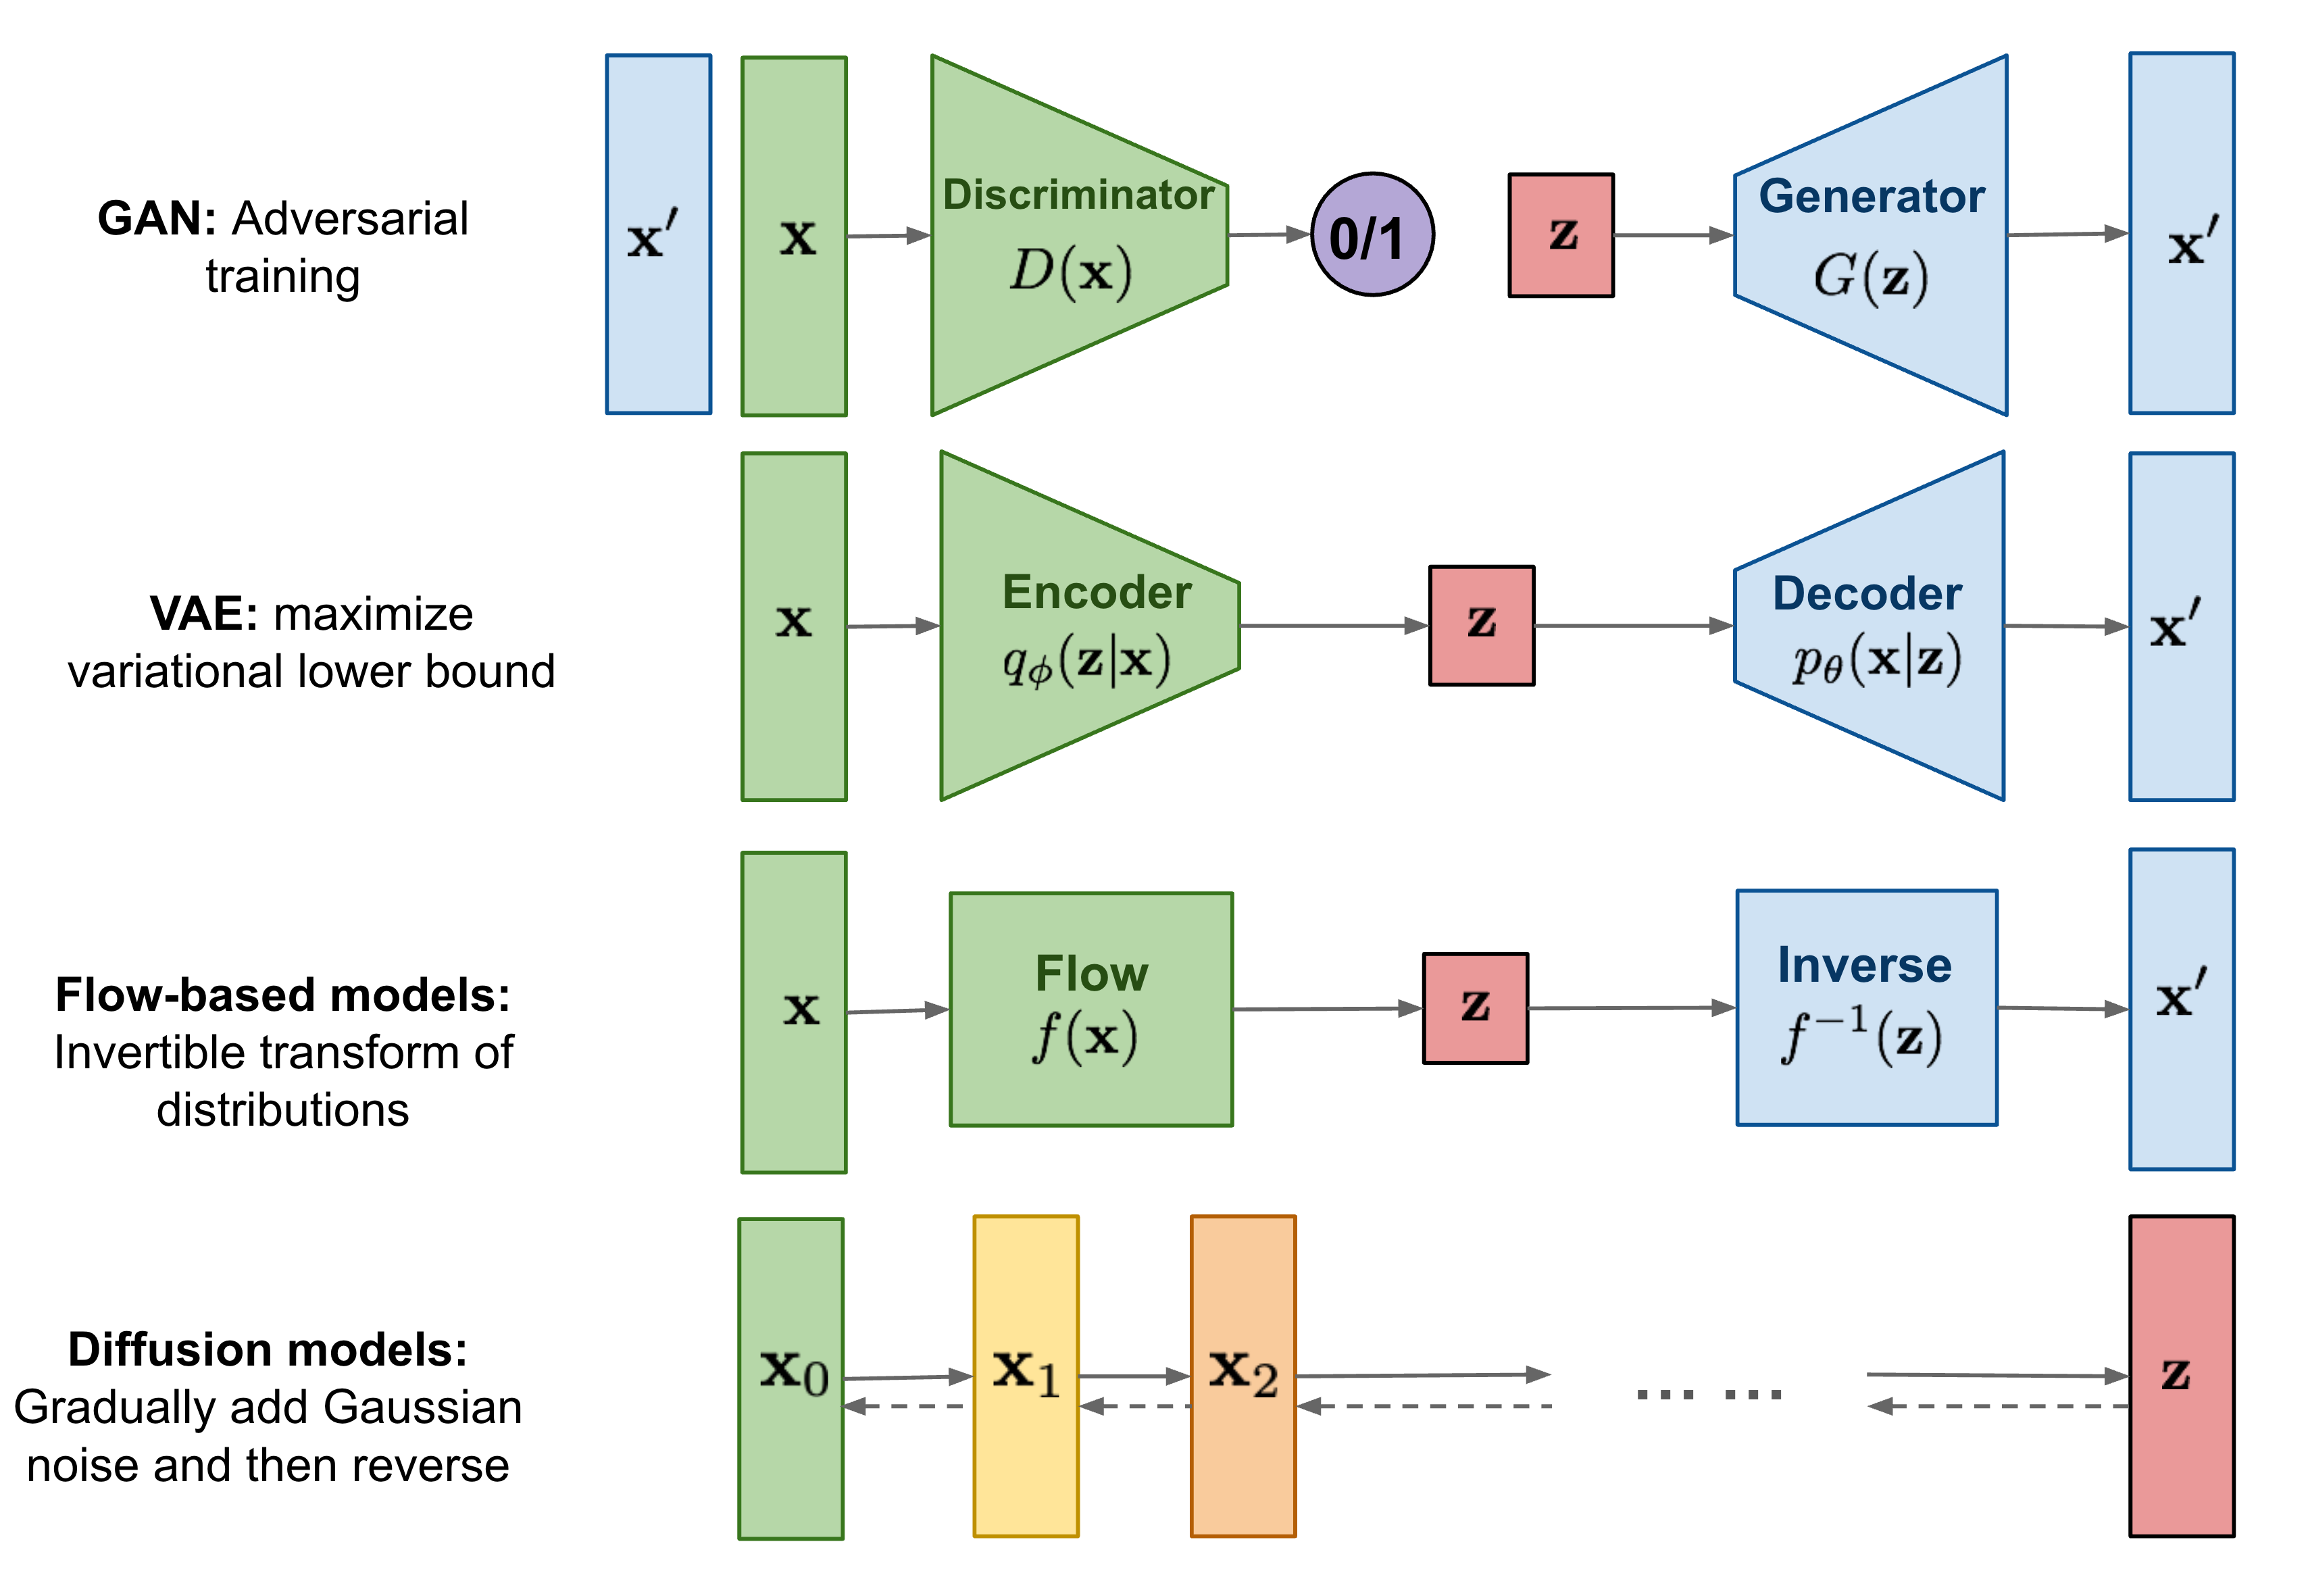
\includegraphics[width=0.9\textwidth]{generative-overview.png}
        \caption{Tổng quát các mô hình sinh}
    \end{figure}
\end{frame}

\begin{frame}
    \begin{figure}[h!]
        \centering
        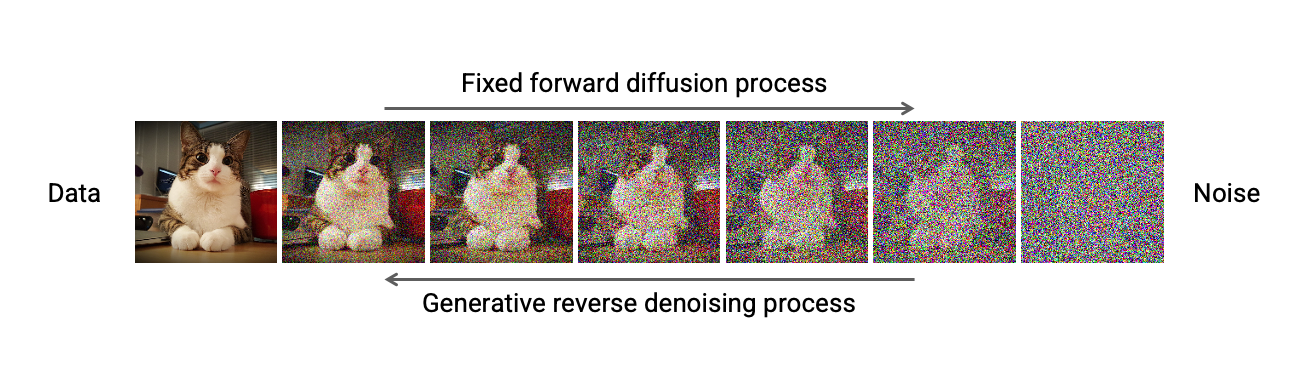
\includegraphics[width=0.9\textwidth]{Fixed_Forward_Diffusion_Process.png}
        \caption{Minh họa một quá trình khuếch tán thuận và khuếch tán ngược}
    \end{figure}
\end{frame}

\begin{frame}
    \begin{equation} \label{eq:ELBO-Maximization}
        \max_{\lbrace \boldsymbol{\mu}_n, \boldsymbol{\Sigma}_n \rbrace_{n=1}^N} L_{\mathrm{elbo}} \Leftrightarrow \min_{\lbrace \boldsymbol{\mu}_n, \boldsymbol{\Sigma}_n \rbrace_{n=1}^N} D_{\mathrm{KL}} \big( q(\boldsymbol{x}_{0:N}) \Vert p(\boldsymbol{x}_{0:N}) \big)
    \end{equation}
    \begin{equation} \label{eq:Optimal-Mean}
        \boldsymbol{\mu}_n^{\ast} (\boldsymbol{x}_n)=\tilde{\boldsymbol{\mu}}_n \Bigg( \boldsymbol{x}_n, \dfrac{1}{\sqrt{\overline{\alpha}_n}} \Big( \boldsymbol{x}_n - \sqrt{\overline{\beta}_n} \mathbb{E}_{q(\boldsymbol{x}_0 \vert \boldsymbol{x}_n)} \lbrack \boldsymbol{\epsilon}_n \rbrack \Big) \Bigg)
    \end{equation}
\end{frame}

\begin{frame}
    \begin{dl}[Nghiệm tối ưu cho bài toán tối ưu hóa chung] \label{dl:Optimal-Solution-To-Joint-Optimization}
        Với ma trận hiệp phương sai có dạng $\boldsymbol{\Sigma}_n (\boldsymbol{x}_n)=\mathrm{diag}\big( \boldsymbol{\sigma}_n (\boldsymbol{x}_n)^2 \big)$.
        Khi đó trung bình tối ưu của bài toán trong công thức \ref{eq:ELBO-Maximization} là $\boldsymbol{\mu}_n^{\ast} (\boldsymbol{x}_n)$ được nêu trong công thức \ref{eq:Optimal-Mean},
        và ma trận hiệp phương sai tối ưu của bài toán trong công thức \ref{eq:ELBO-Maximization} là:

        \begin{equation*}
            \boldsymbol{\sigma}_n^{\ast} (\boldsymbol{x}_n)^2 = \lambda_n^2 \boldsymbol{1} + \gamma_n^2 \dfrac{\overline{\beta}_n}{\overline{\alpha}_n} \big( \mathbb{E}_{q(\boldsymbol{x}_0 \vert \boldsymbol{x}_n)} \lbrack \boldsymbol{\epsilon}_n^2 \rbrack - \mathbb{E}_{q(\boldsymbol{x}_0 \vert \boldsymbol{x}_n)} \lbrack \boldsymbol{\epsilon}_n \rbrack^2 \big)
        \end{equation*}
        với $\boldsymbol{\epsilon}_n = \dfrac{\boldsymbol{x}_n - \sqrt{\overline{\alpha}_n} \boldsymbol{x}_0}{\sqrt{\overline{\beta}_n}}$ là nhiễu được dùng để tạo ra $\boldsymbol{x}_n$ từ $\boldsymbol{x}_0$,
        $(.)^2$ là bình phương từng phần tử của vector, $\boldsymbol{1}$ là vector mà các phần tử đều bằng một và $\gamma_n = \sqrt{\overline{\alpha}_{n-1}} - \sqrt{\overline{\beta}_{n-1} - \lambda_n^2} \sqrt{\dfrac{\overline{\alpha}_n}{\overline{\beta}_n}}$
    \end{dl}
\end{frame}

\begin{frame}
    Ta thu được các lời giải tối ưu bằng cách giải hai bài toán:

    \begin{equation} \label{eq:Arbitrary-Covariance-Optimize-Mean}
        \text{Cho ma trận hiệp phương sai bất kỳ } \boldsymbol{\Sigma}_n, \max_{\lbrace \boldsymbol{\mu}_n \rbrace_{n=1}^N} L_{\mathrm{elbo}}
    \end{equation}

    \begin{equation} \label{eq:Arbitrary-Mean-Optimize-Covariance}
        \text{Cho trung bình bất kỳ } \boldsymbol{\mu}_n, \max_{\lbrace \boldsymbol{\Sigma}_n \rbrace_{n=1}^N} L_{\mathrm{elbo}}
    \end{equation}
\end{frame}

\begin{frame}
    \begin{dl}[Lời giải tối ưu của bài toán tối ưu duy nhất với trung bình] \label{dl:Solely-Optimal-Mean}
        Với ma trận hiệp phương sai bất kỳ $\boldsymbol{\Sigma}_n$,
        trung bình tối ưu của bài toán trong công thức \ref{eq:Arbitrary-Covariance-Optimize-Mean} luôn luôn là trung bình tối ưu trong công thức \ref{eq:Optimal-Mean}:

        \begin{equation*}
            \boldsymbol{\mu}_n^{\ast} (\boldsymbol{x}_n)=\tilde{\boldsymbol{\mu}}_n \Bigg( \boldsymbol{x}_n, \dfrac{1}{\sqrt{\overline{\alpha}_n}} \Big( \boldsymbol{x}_n - \sqrt{\overline{\beta}_n} \mathbb{E}_{q(\boldsymbol{x}_0 \vert \boldsymbol{x}_n)} \lbrack \boldsymbol{\epsilon}_n \rbrack \Big) \Bigg)
        \end{equation*}

        không ảnh hưởng đến $\boldsymbol{\Sigma}_n$.
    \end{dl}
\end{frame}

\begin{frame}
    \begin{equation} \label{eq:Estimated-Optimal-Mean}
        \hat{\boldsymbol{\mu}}_n(\boldsymbol{x}_n)=\tilde{\boldsymbol{\mu}}_n \Bigg( \boldsymbol{x}_n, \dfrac{1}{\sqrt{\overline{\alpha}_n}} \Big( \bold{x}_n - \sqrt{\overline{\beta}_n} \hat{\boldsymbol{\epsilon}}_n(\boldsymbol{x}_n) \Big) \Bigg)
    \end{equation}
\end{frame}

\begin{frame}
    \begin{dl}[Lời giải tối ưu của bài toán tối ưu duy nhất với ma trận hiệp phương sai] \label{dl:Solely-Optimal-Covariance}
        Ta giả định $\boldsymbol{\Sigma}_n = \mathrm{diag} \big( \boldsymbol{\sigma}_n (\boldsymbol{x}_n)^2 \big)$.
        Với trung bình bất kỳ $\boldsymbol{\mu}_n (\boldsymbol{x}_n)$ được tham số hóa bởi mạng dự đoán nhiễu $\hat{\boldsymbol{\epsilon}}_n (\boldsymbol{x}_n)$ như trong công thức \ref{eq:Estimated-Optimal-Mean},
        ma trận hiệp phương sai tối ưu của bài toán trong công thức \ref{eq:Arbitrary-Mean-Optimize-Covariance} là:

        \begin{equation*} \label{eq:Corrected-Optimal-Covariance}
            \begin{aligned}
                \tilde{\boldsymbol{\sigma}}_n^{\ast} (\boldsymbol{x}_n)^2 &= \boldsymbol{\sigma}_n^{\ast} (\boldsymbol{x}_n)^2 + \gamma_n^2 \dfrac{\overline{\beta}_n}{\overline{\alpha}_n} \underbrace{\big( \hat{\boldsymbol{\epsilon}}_n (\boldsymbol{x}_n) - \mathbb{E}_{q(\boldsymbol{x}_0 \vert \boldsymbol{x}_n) \lbrack \boldsymbol{\epsilon}_n \rbrack} \big)^2}_{\mathrm{error}} \\
                &= \lambda_n^2 \boldsymbol{1} + \gamma_n^2 \dfrac{\overline{\beta}_n}{\overline{\alpha}_n} \mathbb{E}_{q(\boldsymbol{x}_0 \vert \boldsymbol{x}_n)} \Big\lbrack \big( \boldsymbol{\epsilon}_n - \hat{\boldsymbol{\epsilon}}_n (\boldsymbol{x}_n) \big)^2 \Big\rbrack
            \end{aligned}
        \end{equation*}

        Với $\boldsymbol{\sigma}_n^{\ast} (\boldsymbol{x}_n)^2$ là ma trận hiệp phương sai tối ưu của bài toán tối ưu hóa chung ở định lý \ref{dl:Optimal-Solution-To-Joint-Optimization},
        $\boldsymbol{\epsilon}_n = \dfrac{\boldsymbol{x}_n - \sqrt{\overline{\alpha}_n} \boldsymbol{x}_0}{\sqrt{\overline{\beta}_n}}$ là nhiễu được dùng để tạo ra $\boldsymbol{x}_n$ từ $\boldsymbol{x}_0$,
        $(.)^2$ là bình phương từng phần tử của vector, $\boldsymbol{1}$ là vector mà các phần tử đều bằng một và $\gamma_n = \sqrt{\overline{\alpha}_{n-1}} - \sqrt{\overline{\beta}_{n-1} - \lambda_n^2} \sqrt{\dfrac{\overline{\alpha}_n}{\overline{\beta}_n}}$.
    \end{dl}
\end{frame}

\begin{frame}
    \begin{algorithm}[H]
        \DontPrintSemicolon
        \KwIn{Mạng dự đoán nhiễu $\hat{\boldsymbol{\epsilon}}_n (\boldsymbol{x}_n)$ và tham số được huấn luyện $\boldsymbol{\theta}$}
        \Repeat{hội tụ}{
            $\boldsymbol{x}_0 \sim q(\boldsymbol{x}_0)$\;
            $n \sim \mathrm{Uniform}\big( \lbrace 1, 2, \dots, N \rbrace\big)$\;
            $\boldsymbol{\epsilon} \sim \mathcal{N}(\boldsymbol{0}, \boldsymbol{I})$\;
            $\boldsymbol{x}_n \gets \sqrt{\overline{\alpha}_n} \boldsymbol{x}_0 + \sqrt{\overline{\beta}_n} \boldsymbol{\epsilon}$\;
            Chỉnh định $\boldsymbol{\theta}$ dựa trên đạo hàm riêng $\nabla_{\boldsymbol{\theta}}  \lVert \boldsymbol{\epsilon}^2 - \hat{\boldsymbol{\epsilon}}_n (\boldsymbol{x}_n) \rVert_2^2$
        }
        \caption{Thủ tục huấn luyện VDM}
        \label{alg:Learning-of-VDM}
    \end{algorithm}
\end{frame}

\begin{frame}
    \begin{algorithm}[H]
        \DontPrintSemicolon
        \KwIn{Mạng dự đoán nhiễu $\hat{\boldsymbol{\epsilon}}_n (\boldsymbol{x}_n)$ và tham số đã được huấn luyện $\boldsymbol{\theta}$}
        $\boldsymbol{x}_N \sim \mathcal{N} (\boldsymbol{0}, \boldsymbol{I})$\;
        \For {$t \gets N, \dots, 1$} {
            \If {$n > 1$} {
                $\boldsymbol{\epsilon} \sim \mathcal{N}(\boldsymbol{0}, \boldsymbol{I})$\;
            } \Else {
                $\boldsymbol{\epsilon} \gets \boldsymbol{0}$\;
            }
        $\boldsymbol{x}_{n-1} \gets \dfrac{1}{\sqrt{\alpha_n}} \Big( \boldsymbol{x}_n - \dfrac{1 - \alpha_n}{\sqrt{1 - \overline{\alpha}_n}} \hat{\boldsymbol{\epsilon}}_n (\boldsymbol{x}_n) \Big) + \lambda_n \boldsymbol{\epsilon}$\;
        }
        \Return{$\boldsymbol{x}_0$}\;
        \caption{Thủ tục lấy mẫu từ một VDM đã được huấn luyện}
        \label{alg:Sampling-of-VDM}
    \end{algorithm}
\end{frame}

\begin{frame}
    \begin{algorithm}[H]
        \DontPrintSemicolon
        \KwIn{Mạng dự đoán bình phương nhiễu (SN) $\boldsymbol{h}_n (\boldsymbol{x}_n)$ và tham số được huấn luyện $\boldsymbol{\phi}_2$}
        \Repeat{hội tụ}{
            $\boldsymbol{x}_0 \sim q(\boldsymbol{x}_0)$\;
            $n \sim \mathrm{Uniform}\big( \lbrace 1, 2, \dots, N \rbrace\big)$\;
            $\boldsymbol{\epsilon}_n \sim \mathcal{N}(\boldsymbol{0}, \boldsymbol{I})$\;
            $\boldsymbol{x}_n \gets \sqrt{\overline{\alpha}_n} \boldsymbol{x}_0 + \sqrt{\overline{\beta}_n} \boldsymbol{\epsilon}_n$\;
            Chỉnh định $\boldsymbol{\phi}_2$ dựa trên đạo hàm riêng $\nabla_{\boldsymbol{\phi}_2}  \lVert \boldsymbol{\epsilon}_n^2 - \boldsymbol{h}_n (\boldsymbol{x}_n) \rVert_2^2$
        }
        \caption{Thủ tục huấn luyện mạng dự đoán nhiễu bình phương (SN)}
        \label{alg:Learning-of-the-SN-prediction-network}
    \end{algorithm}
\end{frame}

\begin{frame}
    \begin{algorithm}[H]
        \DontPrintSemicolon
        \KwIn{Mạng dự đoán nhiễu $\hat{\boldsymbol{\epsilon}}_n (\boldsymbol{x}_n)$ với tham số $\boldsymbol{\phi}_1$ và mạng dự đoán bình phương nhiễu (SN) $\boldsymbol{h}_n (\boldsymbol{x}_n)$ với tham số $\boldsymbol{\phi}_2$}
        $\boldsymbol{x}_N \sim \mathcal{N} (\boldsymbol{0}, \boldsymbol{I})$\;
        \For {$t \gets N, \dots, 1$} {
            \If {$n > 1$} {
                $\boldsymbol{\epsilon} \sim \mathcal{N}(\boldsymbol{0}, \boldsymbol{I})$\;
            } \Else {
                $\boldsymbol{\epsilon} \gets \boldsymbol{0}$\;
            }
            $\hat{\boldsymbol{\sigma}}_n (\boldsymbol{x}_n)^2 \gets \lambda_n^2 \boldsymbol{1} + \gamma_n^2 \dfrac{\overline{\beta}_n}{\overline{\alpha}_n} \big( \boldsymbol{h}_n (\boldsymbol{x}_n) - \hat{\boldsymbol{\epsilon}}_n (\boldsymbol{x}_n)^2 \big)$\;
        $\boldsymbol{x}_{n-1} \gets \dfrac{1}{\sqrt{\alpha_n}} \Big( \boldsymbol{x}_n - \dfrac{1 - \alpha_n}{\sqrt{1 - \overline{\alpha}_n}} \hat{\boldsymbol{\epsilon}}_n (\boldsymbol{x}_n) \Big) + \hat{\boldsymbol{\sigma}}_n (\boldsymbol{x}_n) \odot \boldsymbol{\epsilon}$\;
        }
        \Return{$\boldsymbol{x}_0$}\;
        \caption{Thủ tục lấy mẫu từ một SN-DPM đã được huấn luyện}
        \label{alg:Sampling-of-SN}
    \end{algorithm}
\end{frame}

\begin{frame}
    \begin{algorithm}[H]
        \DontPrintSemicolon
        \KwIn{Mạng dự đoán phần dư nhiễu (NPR) $\boldsymbol{g}_n (\boldsymbol{x}_n)$ và tham số được huấn luyện $\boldsymbol{\phi}_2$;
        mạng dự đoán nhiễu đã được tiền huấn luyện $\hat{\boldsymbol{\epsilon}}_n (\boldsymbol{x}_n)$}
        \Repeat{hội tụ}{
            $\boldsymbol{x}_0 \sim q(\boldsymbol{x}_0)$\;
            $n \sim \mathrm{Uniform}\big( \lbrace 1, 2, \dots, N \rbrace\big)$\;
            $\boldsymbol{\epsilon}_n \sim \mathcal{N}(\boldsymbol{0}, \boldsymbol{I})$\;
            $\boldsymbol{x}_n \gets \sqrt{\overline{\alpha}_n} \boldsymbol{x}_0 + \sqrt{\overline{\beta}_n} \boldsymbol{\epsilon}_n$\;
            Chỉnh định $\boldsymbol{\phi}_2$ dựa trên đạo hàm riêng $\nabla_{\boldsymbol{\phi}_2}  \lVert \big( \boldsymbol{\epsilon}_n - \hat{\boldsymbol{\epsilon}}_n (\boldsymbol{x}_n) \big)^2 - \boldsymbol{g}_n (\boldsymbol{x}_n) \rVert_2^2$
        }
        \caption{Thủ tục huấn luyện mạng dự đoán phần dư nhiễu (NPR)}
        \label{alg:Learning-of-the-NPR-prediction-network}
    \end{algorithm}
\end{frame}


\begin{frame}
    \begin{algorithm}[H]
        \DontPrintSemicolon
        \KwIn{Mạng dự đoán nhiễu $\hat{\boldsymbol{\epsilon}}_n (\boldsymbol{x}_n)$ với tham số $\boldsymbol{\phi}_1$ và mạng dự đoán phần dư nhiễu (NPR) $\boldsymbol{g}_n (\boldsymbol{x}_n)$ với tham số $\boldsymbol{\phi}_2$}
        $\boldsymbol{x}_N \sim \mathcal{N} (\boldsymbol{0}, \boldsymbol{I})$\;
        \For {$t \gets N, \dots, 1$} {
            \If {$n > 1$} {
                $\boldsymbol{\epsilon} \sim \mathcal{N}(\boldsymbol{0}, \boldsymbol{I})$\;
            } \Else {
                $\boldsymbol{\epsilon} \gets \boldsymbol{0}$\;
            }
            $\hat{\tilde{\boldsymbol{\sigma}}}_n (\boldsymbol{x}_n)^2 \gets \lambda_n^2 \boldsymbol{1} + \gamma_n^2 \dfrac{\overline{\beta}_n}{\overline{\alpha}_n} \boldsymbol{g}_n (\boldsymbol{x}_n)$\;
        $\boldsymbol{x}_{n-1} \gets \dfrac{1}{\sqrt{\alpha_n}} \Big( \boldsymbol{x}_n - \dfrac{1 - \alpha_n}{\sqrt{1 - \overline{\alpha}_n}} \hat{\boldsymbol{\epsilon}}_n (\boldsymbol{x}_n) \Big) + \hat{\tilde{\boldsymbol{\sigma}}}_n (\boldsymbol{x}_n) \odot \boldsymbol{\epsilon}$\;
        }
        \Return{$\boldsymbol{x}_0$}\;
        \caption{Thủ tục lấy mẫu từ một NPR-DPM đã được huấn luyện}
        \label{alg:Sampling-of-NPR}
    \end{algorithm}
\end{frame}
\begin{frame}
    \begin{table}[h!]
        %\small
        %\centering
        \caption{Bảng kết quả khoảng cách FID. Tất cả các kết quả đều với cấu hình quỹ đạo chẵn (ET). A-DPM ký hiệu của Analytic-DPM. 
        Ta cần chú ý rằng chi phí thời gian tăng thêm của mạng dự đoán phần dư nhiễu NPR hoặc mạng dự đoán bình phương nhiễu SN là không đáng kể trên tập CIFAR10, CelebA 64x64 và khoảng 4.5 \% trên tập ImageNet 64x64
        (chi tiết ở phụ lục \ref{Appen:Subsection:Details-of-Memory-and-Time-Cost}). Ta có thể sử dụng số bước để so sánh tính hiệu quả của các phương pháp}
        \resizebox{\columnwidth}{!}{
            \begin{tabular}{ lrrrrrrrrrrrrr  }
                \hline
                \multirow{2}{*}{\# Số bước $K$} & \multicolumn{6}{c}{CIFAR10 (LS)} & & \multicolumn{6}{c}{CIFAR10 (CS)} \\ \cline{2-7} \cline{9-14}
                & 10 & 25 & 50 & 100 & 200 & 1000 & & 10 & 25 & 50 & 100 & 200 & 1000 \\
                \hline
                DDPM, $\tilde{\beta}_n$ & 44.45 & 21.83 & 15.21 & 10.94 & 8.23 & 5.11 &  & 34.76 & 16.18 & 11.11 & 8.38 & 6.66 & 4.92 \\
                DDPM, $\beta_n$ & 233.41 & 125.05 & 66.28 & 31.36 & 12.96 & \textbf{3.04} & & 205.31 & 84.71 & 37.35 & 14.81 & 5.74 & \textbf{3.34} \\
                A-DDPM & 34.26 & 11.60 & 7.25 & 5.40 & 4.01 & 4.03 & & 22.94 & 8.50 & 5.50 & 4.45 & 4.04 & 4.31 \\
                NPR-DDPM & 32.35 & 10.55 & 6.18 & 4.52 & 3.57 & 4.10 & & 19.94 & 7.99 & 5.31 & 4.52 & 4.10 & 4.27 \\
                SN-DDPM & \textbf{24.06} & \textbf{6.91} & \textbf{4.63} & \textbf{3.67} & \textbf{3.31} & 3.65 & & \textbf{16.33} & \textbf{6.05} & \textbf{4.17} & \textbf{3.83} & \textbf{3.72} & 4.07 \\
                \hline
                DDIM & 21.31 & 10.70 & 7.74 & 6.08 & 5.07 & 4.13 & & 34.34 & 16.68 & 10.48 & 7.94 & 6.69 & 4.89 \\
                A-DDIM & 14.00 & 5.81 & 4.04 & 3.55 & 3.39 & 3.74 & & 26.43 & 9.96 & 6.02 & 4.88 & 4.92 & 4.66 \\
                NPR-DDIM & 13.34 & 5.38 & 3.95 & 3.53 & 3.42 & 3.72 & & 22.81 & 9.47 & 6.04 & 5.02 & 5.06 & 4.62 \\
                SN-DDIM & \textbf{12.19} & \textbf{4.28} & \textbf{3.39} & \textbf{3.23} & \textbf{3.22} & \textbf{3.65} & & \textbf{17.90} & \textbf{7.36} & \textbf{5.16} & \textbf{4.63} & \textbf{4.63} & \textbf{4.51} \\
                \hline
            \end{tabular}
        }
        \resizebox{\columnwidth}{!} {
            \begin{tabular}{ lrrrrrrrrrrrrr  }
                \hline
                \multirow{2}{*}{\# Số bước $K$} & \multicolumn{6}{c}{CelebA 64x64} & & \multicolumn{6}{c}{ImageNet 64x64} \\ \cline{2-7} \cline{9-14}
                & 10 & 25 & 50 & 100 & 200 & 1000 & & 25 & 50 & 100 & 200 & 400 & 4000 \\
                \hline
                DDPM, $\tilde{\beta}_n$ & 36.69 & 24.46 & 18.96 & 14.31 & 10.48 & 5.95 & & 29.21 & 21.71 & 19.12 & 17.81 & 17.48 & 16.55 \\
                DDPM, $\beta_n$ & 294.79 & 115.69 & 53.39 & 25.65 & 9.72 & \textbf{3.16} & & 170.28 & 83.86 & 45.04 & 28.39 & 21.38 & 16.38 \\
                A-DDPM & 28.99 & 16.01 & 11.23 & 8.08 & 6.51 & 5.21 & & 32.56 & 22.45 & 18.80 & 17.16 & 16.40 & 16.34 \\
                NPR-DDPM & 28.37 & 15.74 & 10.89 & 8.23 & 7.03 & 5.33 & & 28.27 & 20.89 & 18.06 & 16.96 & \textbf{16.32} & 16.38 \\
                SN-DDPM & \textbf{20.60} & \textbf{12.00} & \textbf{7.88} & \textbf{5.89} & \textbf{5.02} & 4.42 & & \textbf{27.58} & \textbf{20.74} & \textbf{18.04} & \textbf{16.61} & 16.37 & \textbf{16.22} \\
                \hline
                DDIM & 20.54 & 13.45 & 9.33 & 6.60 & 4.96 & 3.40 & & 26.06 & 20.10 & 18.09 & 17.84 & 17.74 & 19.00 \\
                A-DDIM & 15.62 & 9.22 & 6.13 & 4.29 & 3.46 & 3.13 & & \textbf{25.98} & \textbf{19.23} & 17.73 & 17.49 & 17.44 & 18.98 \\
                NPR-DDIM & 14.98 & 8.93 & 6.04 & 4.27 & 3.59 & 3.15 & & 28.84 & 19.62 & 17.63 & 17.42 & 17.30 & 18.91 \\
                SN-DDIM & \textbf{10.20} & \textbf{5.48} & \textbf{3.83} & \textbf{3.04} & \textbf{2.85} & \textbf{2.90} & & 28.07 & 19.38 & \textbf{17.53} & \textbf{17.23} & \textbf{17.23} & \textbf{18.89} \\
                \hline
            \end{tabular}
        }
        \begin{center}
            \resizebox{9.5cm}{!}{
                \begin{tabular}{ lrrrrrr  }
                    \hline
                    \multirow{2}{*}{\# Số bước $K$} & \multicolumn{6}{c}{CIFAR10 (VP SDE)} \\ \cline{2-7}
                    & 10 & 25 & 50 & 100 & 200 & 1000 \\
                    \hline
                    Euler-Maruyama & 292.20 & 170.17 & 90.79 & 47.46 & 21.92 & \textbf{2.55} \\
                    Ancestral-Sampling & 235.28 & 129.29 & 68.52 & 31.99 & 12.81 & 2.72 \\
                    Probabity Flow & 107.74 & 21.34 & 7.78 & 4.33 & 3.27 & 2.82 \\
                    A-DPM & 35.10 &  11.57 & 6.54 & 4.71 & 3.61 & 2.98 \\
                    NPR-DPM & 33.70 & 10.44 & 5.83 & 3.97 & 3.05 & 3.04 \\
                    SN-DPM & \textbf{25.30} & \textbf{7.34} & \textbf{4.46} & \textbf{3.27} & \textbf{2.83} & 2.71 \\
                    \hline
                \end{tabular}
            }
        \end{center}
        \label{table:FID-CIFAR10}
    \end{table}
\end{frame}

\end{document}